% !TEX program = xelatex
\documentclass[11pt,a4paper]{article}

\usepackage[a4paper,margin=22mm]{geometry}
\usepackage{xeCJK}
\usepackage{fontspec}
\usepackage{amsmath,amssymb}
\usepackage{booktabs}
\usepackage{tabularx}
\usepackage{array}
\usepackage{enumitem}
\usepackage{xcolor}
\usepackage{graphicx}
\usepackage{hyperref}

\setCJKmainfont{Hiragino Mincho ProN}
\setCJKsansfont{Hiragino Sans}
\setCJKmonofont{Hiragino Sans}
\setmonofont{Menlo}[Scale=0.82]

\xeCJKDeclareCharClass{CJK}{"2460 -> "24FF, "2013 -> "2015, "2018 -> "201F, "2026, "2500}

\hypersetup{colorlinks=true, linkcolor=black, urlcolor=blue!60!black,
  pdftitle={DOFBOT × Xinu メッシュ 6台 システム設計 (第2版)},
  pdfauthor={児玉靖司}}

\newcommand{\code}[1]{\texttt{#1}}
\newcommand{\prob}[1]{\textbf{\textcolor{red!55!black}{#1}}}
\newcommand{\good}[1]{\textbf{\textcolor{green!45!black}{#1}}}

\title{DOFBOT × Xinu メッシュ 6 台\\ \large システム全体設計（第 2 版）\\
       \normalsize Capability 推論による役割分担・冗長化・アクター移動}
\author{}
\date{2026年7月21日}

\begin{document}
\maketitle

\begin{abstract}
\noindent
第 1 版は 12 台を静的な ServoMotor/ServoSensor 対として扱い、当初構想の中核である
\textbf{Capability 推論による役割分担・冗長性・アクターの動的移動}を設計に反映して
いなかった。本版はそれを中心に据えて構成し直す。

中心となる主張は 1 つ。\good{アクターの効果集合から、配置・複製可否・
フェイルオーバの手順が機械的に決まる}。純粋なアクターは自由に複製でき、
外部作用を持つアクターは\textbf{同時に 1 つしか存在してはならない} ---
つまりフェイルオーバとは Capability の移譲そのものである。

6 軸に 6 台を 1 対 1 で割り当て、\good{冗長性は待機機ではなく、
故障時に空いているノードへアクターを転送することで確保する}。
6 台で全軸を担当でき、当初構想の中核である\textbf{アクターの動的移動が
そのまま可用性の機構になる}。

ただし現状 2 つの障害がある。\prob{効果格子が「自己状態の変更」と「外部への作用」を
同一視している}こと、そして\prob{実測レイテンシの裾が秒単位}であること。
前者は型システムの小さな拡張で解ける。後者は解けないので、
\textbf{フェイルオーバは秒オーダである}という前提で安全性を設計する。
\end{abstract}

\section{当初構想と第 1 版のずれ}

当初の構想は次のとおりであった。

\begin{quote}
AIPL のアクターを生成し、Capability 推論で役割分担させ、6 軸に対して 2 台ずつ
Xinu を用意して冗長性を持たせ、アクターの移動を動的に行い、全体として効率の良い
リアルタイム OS とする。
\end{quote}

第 1 版はこのうち「6 軸 $\times$ 2 台」だけを写し取り、残りを落としていた。
Capability は役割の\textbf{説明}に使われるだけで設計判断に効いておらず、
冗長性は台数の話に留まり、アクター移動に至っては触れていない。本版で立て直す。

\section{現物 --- CG シミュレータ}

\begin{figure}[htbp]
\centering
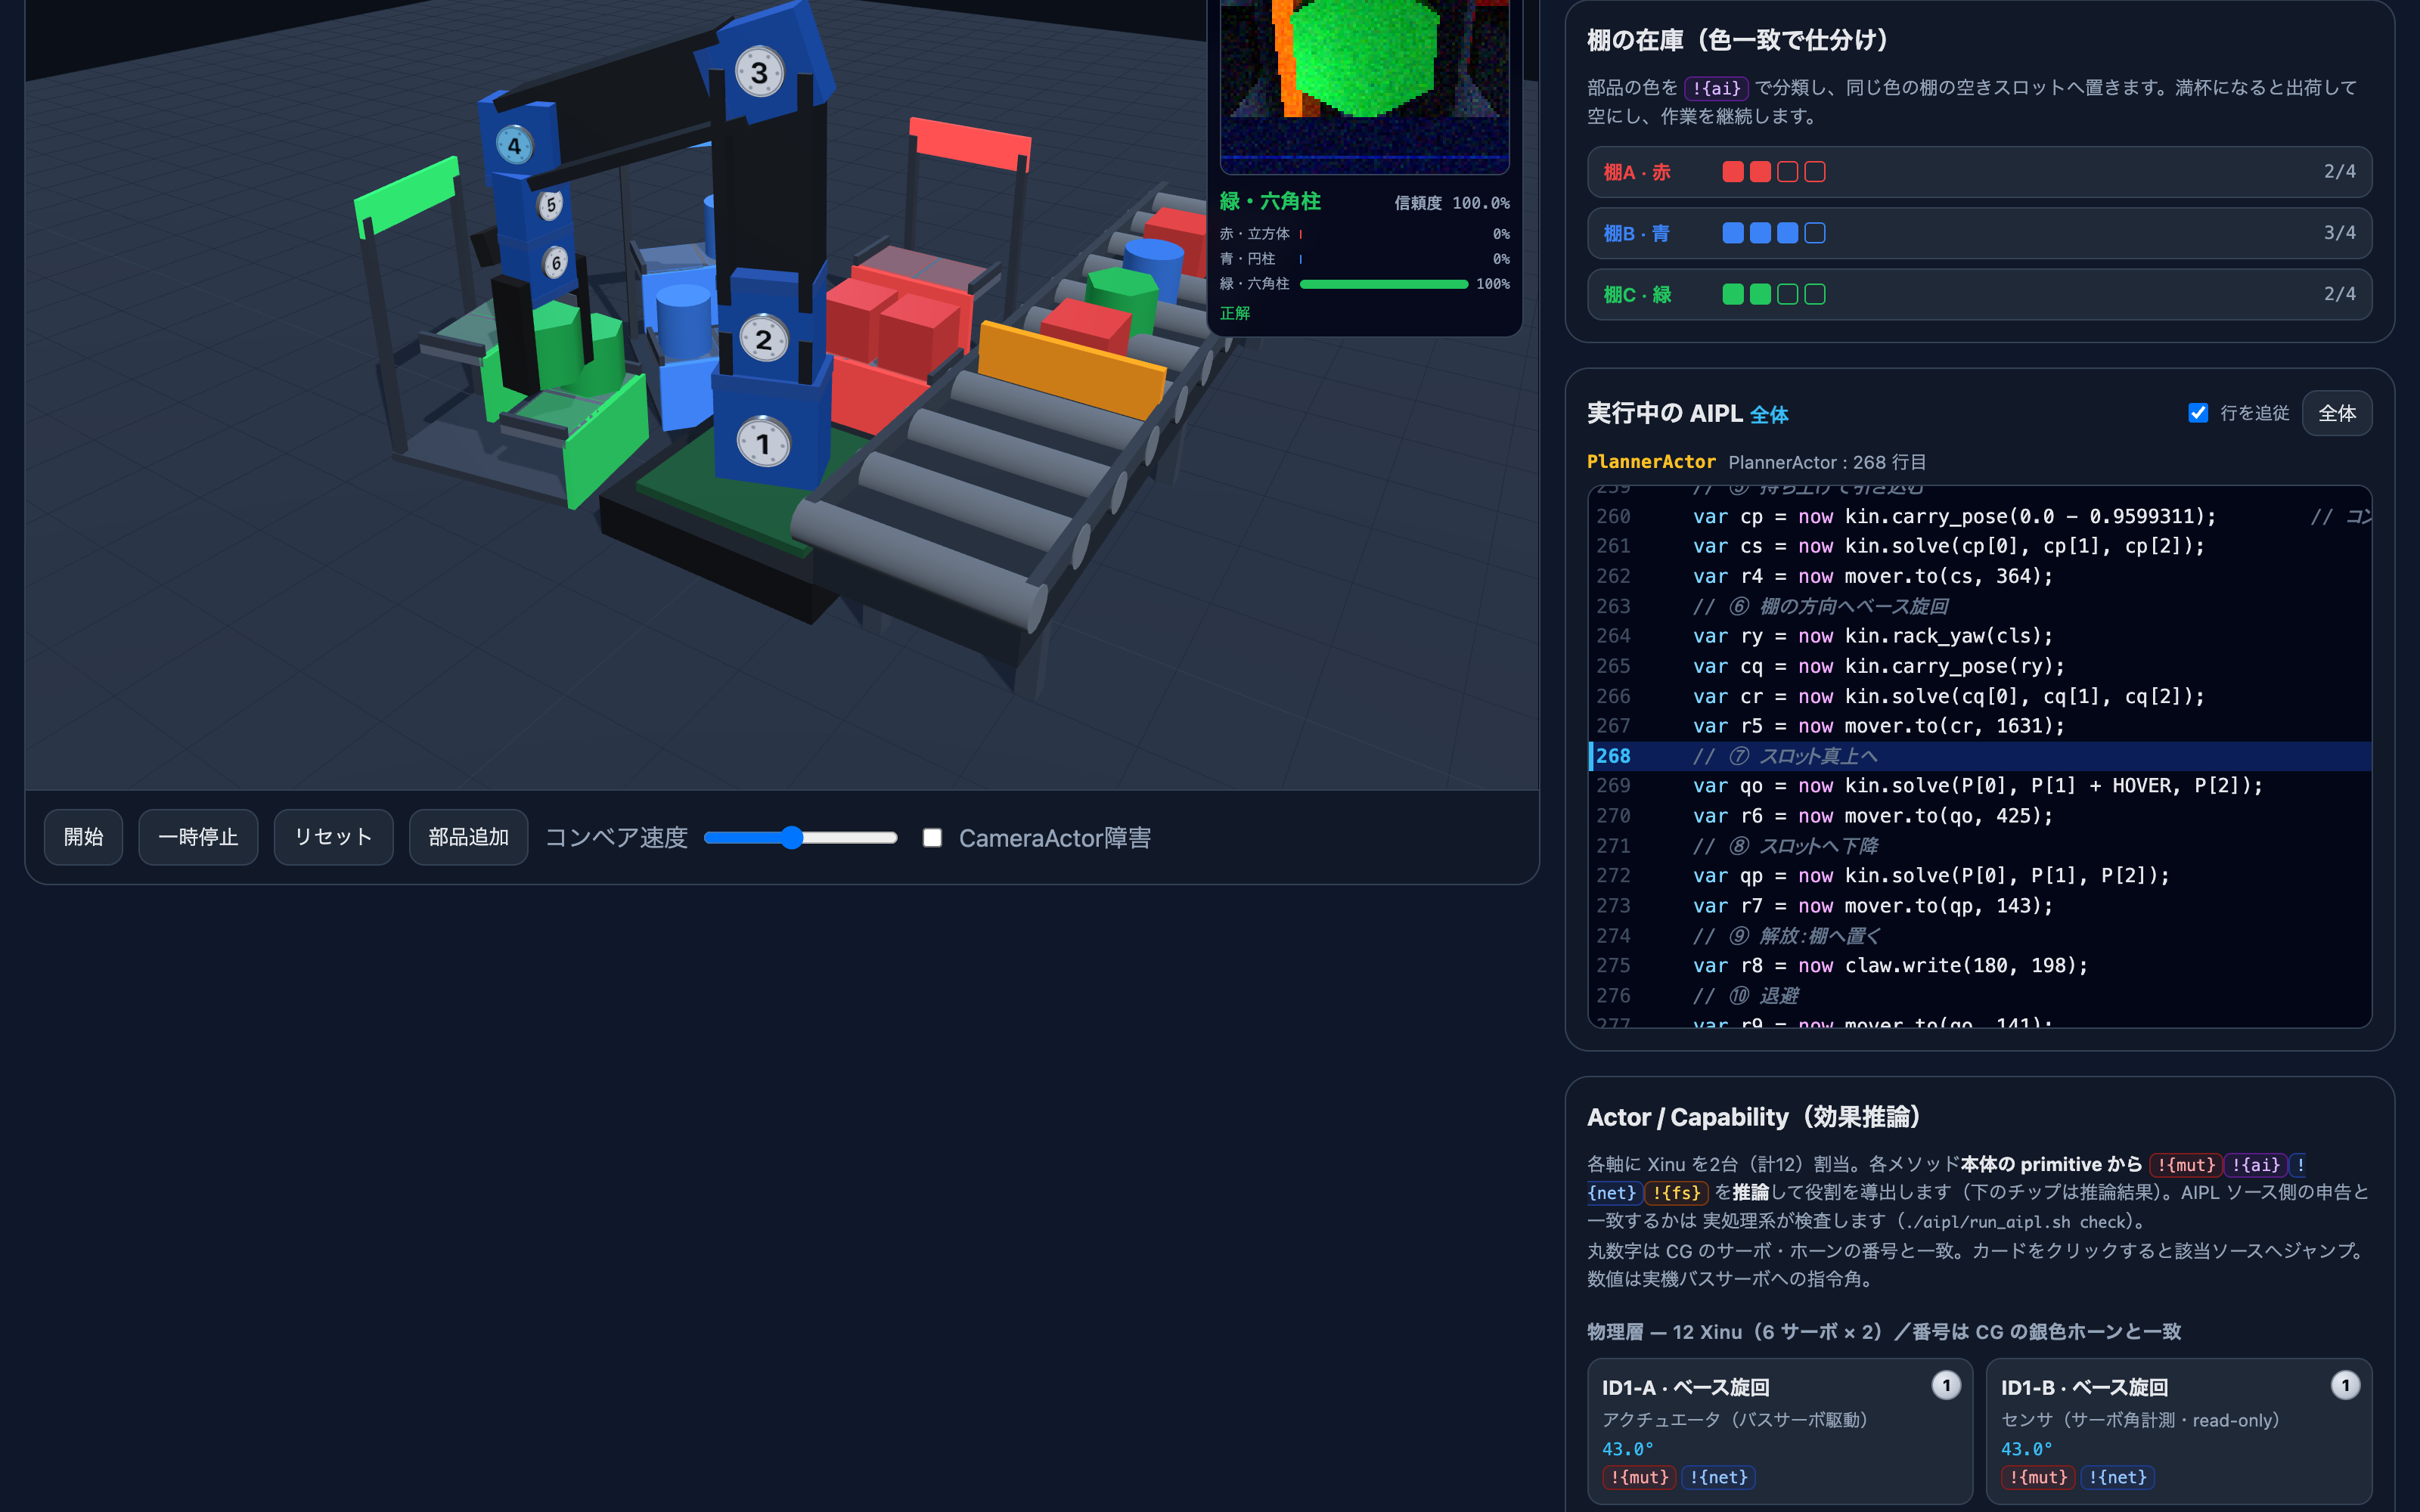
\includegraphics[width=\textwidth]{fig/sim_cg.png}
\caption{DOFBOT ライン作業シミュレータ（\code{:8022}）。2026-07-21 実行、
\code{node test/verify.mjs} で全項目合格した状態。左は 3D の作業セル
（銀色ホーンの丸数字が実機サーボ ID 1--6 に対応）、右上は手首カメラの映像と
TinyML の分類結果（緑・六角柱 100\,\%）、中央右は\textbf{実行中の AIPL ソースで、
現在実行している行が強調表示}される（\code{PlannerActor} 268 行目）、
右下が\textbf{Actor / Capability パネル}で、各アクターの効果推論結果
\code{!\{mut\}} \code{!\{net\}} がチップとして表示される。}
\label{fig:sim}
\end{figure}

図~\ref{fig:sim} が本設計の出発点である。重要なのは右下のパネルで、
\textbf{効果はソースに書かれたものではなく推論結果}であり、
実処理系の \code{--type-check} が申告と実体の一致を検査する。
本設計はこのパネルが示す情報だけから配置・複製・フェイルオーバを導く。

シミュレータは 6 軸それぞれに soft-Xinu を 2 台、計 12 個のアクターを走らせている。
\textbf{実機 6 台は、このうち 6 個を置き換える}という位置づけになる。

\section{6 台の割当 --- 1 軸 1 台}

\textbf{6 軸に 6 台を 1 対 1 で割り当てる。} アーム全軸が実機 Xinu で駆動される。

\begin{center}\small
\begin{tabular}{@{}l l l l@{}}
\toprule
\textbf{ノード} & \textbf{担当} & \textbf{役割} & \textbf{保持する効果}\\
\midrule
1 & ID1 ベース旋回 & \code{ServoMotor} & \code{!\{act, mut, net\}}\\
2 & ID2 肩         & \code{ServoMotor} & \code{!\{act, mut, net\}}\\
3 & ID3 肘         & \code{ServoMotor} & \code{!\{act, mut, net\}}\\
4 & ID4 手首ピッチ & \code{ServoMotor} & \code{!\{act, mut, net\}}\\
5 & ID5 手首回転   & \code{ServoMotor} & \code{!\{act, mut, net\}}\\
6 & ID6 グリッパ   & \code{ServoMotor} & \code{!\{act, mut, net\}}\\
\bottomrule
\end{tabular}
\end{center}

対応する \code{ServoSensor} 6 個は CG 側の soft-Xinu が担う。
純粋アクター（\code{Kinematics}）は効果を持たないので\textbf{6 台すべてに複製}する
（第~\ref{sec:rules} 節）。

\textbf{冗長性は待機機を置くのではなく、いざというときに空いているノードへ
アクターを転送して確保する。} 6 台すべてが実務に就いているので、
専用の待機機は存在しない。故障時には、\textbf{生き残ったノードのうち余裕のあるものが
失われたアクターを引き受ける}。次節で成立条件を示す。

台数効果の測定点は \textbf{2 / 4 / 6} の 3 点とする。担当する軸数を増やしながら
同じ作業のサイクル時間を測れば傾向が取れる。1 点では傾向を主張できないので、
\textbf{6 台は「3 点が取れる最小」}でもある。

\section{Capability から配置と冗長化を導く}

\subsection{効果は宣言ではなく推論される}

AIPL の Capability はソースに書くものではない。各メソッド本体の一次作用を
効果推論が走査して \code{!\{mut, net, ai, fs\}} を導出し、
\code{--type-check} が申告と実体の食い違いを検出する。
現在の割当は次のとおり。

\begin{center}\small
\begin{tabularx}{\textwidth}{@{}l l X@{}}
\toprule
\textbf{一次作用} & \textbf{効果} & \textbf{意味}\\
\midrule
\code{Arm\_serial\_servo\_write} & \code{mut} & 実機バスサーボの駆動\\
\code{Arm\_serial\_servo\_read}  & なし & 計測のみ。何も動かさない\\
\code{tinyml\_infer}            & \code{ai} & ローカル推論。\code{net} を伴わない = 機外へ出ない\\
\code{tinyml\_load} / \code{write\_file} & \code{fs} & 記憶装置\\
\code{send} / \code{now} / \code{reply} & \code{net} & メッセージ\\
\bottomrule
\end{tabularx}
\end{center}

これは強力である。\code{ServoSensor} は \code{Arm\_serial\_servo\_write} を呼ぶ場所が
ソース中のどこにも無いため、\good{型によって物理的に駆動できないことが保証される}。
最小権限が設計意図ではなく検査可能な性質になっている。

\subsection{発見: 効果格子が作用と状態変更を同一視している}

しかし配置の自動導出には足りない。現在のクラスの効果は次のようになる。

\begin{center}\small
\begin{tabular}{@{}l l l@{}}
\toprule
\textbf{クラス} & \textbf{効果} & \textbf{外部への作用}\\
\midrule
\code{ServoMotor}       & \code{!\{mut, net\}} & \good{あり（サーボを回す）}\\
\code{ShelfActor}       & \code{!\{mut, net\}} & なし（自分の在庫表を書くだけ）\\
\code{ConveyorActor}    & \code{!\{mut, net\}} & あり（ストッパを開閉）\\
\code{ArmMover}         & \code{!\{net\}}      & なし\\
\code{Kinematics}       & \code{!\{net\}}      & なし（純計算 + \code{reply}）\\
\code{RecognitionActor} & \code{!\{ai, net\}}  & なし\\
\code{SafetyActor}      & \code{!\{fs, mut, net\}} & なし\\
\bottomrule
\end{tabular}
\end{center}

\prob{\code{ServoMotor} と \code{ShelfActor} は効果集合が同一である。}
一方は実機を動かし、他方は自分のフィールドを書くだけなのに区別が付かない。
ソース中のコメント自身が「\code{bind()} の \code{mut} は自分のフィールド \code{id} への
代入であって、サーボ駆動ではない」と断っており、この曖昧さは認識されている。

配置と複製の規則を効果から導くには、この 2 つを分ける必要がある。

\begin{center}\small
\begin{tabularx}{\textwidth}{@{}l l X@{}}
\toprule
\textbf{提案する効果} & \textbf{意味} & \textbf{導かれる規則}\\
\midrule
\code{mut} & 自分の状態を書く & 複製可（各複製が自分の状態を持つ）\\
\good{\code{act}} & \textbf{外部世界へ作用する} & \prob{同時に 1 つだけ}。配置はその機器に繋がったノードに限定\\
\bottomrule
\end{tabularx}
\end{center}

\code{Arm\_serial\_servo\_write} と \code{conveyor\_stopper} を \code{act} に移すだけで、
\code{ServoMotor}/\code{ConveyorActor} と \code{ShelfActor} が型で分かれる。
\textbf{これは小さな変更だが、以降の設計全体がこの区別の上に載る。}

\subsection{効果集合から決まる規則}\label{sec:rules}

\begin{center}\small
\begin{tabularx}{\textwidth}{@{}l l l X@{}}
\toprule
\textbf{効果} & \textbf{配置} & \textbf{複製} & \textbf{根拠}\\
\midrule
なし（純粋） & どこでも & \good{自由} & 副作用が無いので二重実行が無害。冗長化の費用がゼロ\\
\code{!\{net\}} & どこでも & 可（冪等なら） & 重複メッセージを受け手が吸収できる必要\\
\code{!\{mut\}} & どこでも & 可 & 各複製が独立した状態を持つ\\
\code{!\{ai\}} & 重みを持つノード & 可 & 推論は決定的。機外へ出ない\\
\code{!\{fs\}} & 記憶装置を持つノード & 不可 & 書き込みが競合する\\
\good{\code{!\{act\}}} & \textbf{その機器に繋がったノード} & \prob{不可（厳密に 1 つ）} & 二重駆動は物理的に危険\\
\bottomrule
\end{tabularx}
\end{center}

\code{Kinematics} は効果を持たないので\textbf{全ノードに複製してよい}。
逆運動学を 6 台のどこで解いても同じ答えが出るので、冗長化は無料である。
一方 \code{ServoMotor} は \code{act} を持つので\textbf{厳密に 1 つ}でなければならない。

\section{冗長化 --- 空きノードへのアクター転送}

専用の待機機を置かず、\textbf{故障時に失われたアクターを別のノードへ転送する}ことで
冗長性を確保する。6 台すべてが実務に就いたまま冗長化できるのが利点である。

\subsection{成立条件 1 --- \code{act} が場所に縛られないこと}

第~\ref{sec:rules} 節の規則では、\code{act} を持つアクターの配置は
「その機器に繋がったノード」に限定される。もしこの制約が効くなら、
\code{ServoMotor} は特定のノードから動かせず、転送による冗長化は\textbf{成立しない}。

\good{本構成では制約が効かない。} サーボバスはアーム内蔵 Pi（L0）の背後にあり、
Xinu 側はネットワーク越しに駆動指令を送る。\textbf{どのノードからでも同じように
届くので、\code{act} の配置は場所に依存しない。}

\prob{これは本構成に固有の性質であって、一般的な性質ではない。}
別紙で提案した「スマートジョイント」構成 --- 各関節のボードが自分のサーボに
直接配線される --- では \code{act} は物理的に場所に縛られ、
\textbf{この転送方式は使えなくなる}。冗長化は待機機方式へ戻る必要がある。
設計を実機構成ごと切り替えるときに、ここを見落としてはならない。

\subsection{成立条件 2 --- 状態が機器から読み直せること}

転送先のノードは失われたアクターの状態を持っていない。
待機機方式なら副が鏡像を保持しているので転送が要らないが、
今回は\textbf{状態をどこかから復元しなければならない}。
今日の実測ではメッシュの裾が秒単位あるため、故障したノードから取りに行く設計は
そもそも成立しない（相手は落ちている）。

\good{\code{ServoMotor} の状態は機器から読み直せる。}
このアクターが持つのは \code{id} と \code{pos} だけで、
\code{pos} は \code{Arm\_serial\_servo\_read} で現在角として取得できる。
つまり\textbf{状態はハードウェアの側にある実体の写しにすぎず、転送先で再取得できる}。

\begin{center}\small
\begin{tabularx}{\textwidth}{@{}l l X@{}}
\toprule
\textbf{アクター} & \textbf{状態の復元} & \textbf{転送可否}\\
\midrule
\code{ServoMotor} & \good{機器から読み直す} & \good{可}（状態転送が不要）\\
\code{Kinematics} & 状態を持たない & \good{可}（そもそも複製済み）\\
\code{ShelfActor} & \prob{機器に無い} & 要状態転送。棚の在庫は外から読めない\\
\code{SafetyActor} & \code{fs} に残る & 記憶装置を持つノードに限定\\
\bottomrule
\end{tabularx}
\end{center}

\textbf{したがって転送方式が無条件に使えるのは \code{ServoMotor} と純粋アクターであり、
それ以外は別途手当てが要る。} 6 軸の駆動という本題に関しては十分である。

\subsection{成立条件 3 --- 生き残りに余裕があること}

6 台すべてが 1 軸を担当しているので、\textbf{空いているノードは存在しない}。
故障時は\textbf{生き残ったノードのいずれかが 2 軸を兼務する}ことになる。

\begin{center}
\begin{tabular}{@{}l l l@{}}
\toprule
\textbf{状態} & \textbf{ノード数} & \textbf{担当}\\
\midrule
正常 & 6 & 各ノード 1 軸\\
1 台故障 & 5 & 1 台が 2 軸、残り 4 台が 1 軸\\
2 台故障 & 4 & 2 台が 2 軸、残り 2 台が 1 軸\\
\bottomrule
\end{tabular}
\end{center}

\prob{これは「各ノードが 2 軸ぶんの実時間予算を持つこと」を要求する。}
成立するかは実測でしか分からない。10\,Hz 制御なら 1 軸あたりの処理は
推論を含めても 1\,ms 未満（第~\ref{sec:rt} 節）なので余裕はあるはずだが、
\textbf{兼務時の締切遵守率を測るまでは仮定である}。
これは 6 台構成で最初に測るべき数字の 1 つである。

\subsection{転送の手順 --- \code{act} は期限付きリース}

\code{act} は厳密に 1 つという規則があるので、転送は\textbf{排他的な移譲}でなければ
ならない。分断時に新旧 2 つの \code{ServoMotor} が同じ軸を駆動する事態は物理的に危険である。
そこで \code{act} を\textbf{期限付きリース}として扱う。

\begin{enumerate}[leftmargin=1.6em,itemsep=3pt]
\item 保持者は周期 $T_r$ でリースを更新する。
\item 保持者が $T_e$ 以内に更新できなければ、\textbf{自力で駆動を停止する}
      （ネットワーク不要。ローカルの時計だけで判定できる）。
\item 協調役が $T_e$ 経過を観測し、余裕のあるノードを選んで
      \code{/actor/load} でコードを送り込む。
\item 転送先が \code{Arm\_serial\_servo\_read} で現在角を読み、状態を復元する。
\item 転送先が \code{act} リースを取得し、駆動を開始する。
\end{enumerate}

\prob{手順 2 が安全性の要である。} 分断された旧保持者が「自分はまだ担当だ」と
思い込んで駆動し続けることを、ネットワークに頼らず防ぐ。分散ロックのリースと同じ論法で、
\textbf{Capability がリソースではなく期限付き権限であることを利用している。}

\subsection{タイミング --- 秒オーダであることを認める}

\begin{center}
\begin{tabular}{@{}l r l@{}}
\toprule
\textbf{量} & \textbf{値} & \textbf{根拠}\\
\midrule
HELLO 周期 & 2\,s & \code{device/wifi/wifi.c}（現行実装）\\
往復レイテンシ p99 & 84--1019\,ms & 本日実測（Pi 5 / Pi 3、Pi 3 は \code{NTCP} 修正後）\\
リース更新 $T_r$ & $\ge$1\,s & p99 の裾を吸収する\\
リース期限 $T_e$ & $\ge$3\,s & $T_r$ の 3 倍。誤検知を避ける\\
コード転送 \code{/actor/load} & \prob{未測定} & AIPL → C JIT + POST。実測が要る\\
状態の読み直し & $\sim$1 往復 & \code{Arm\_serial\_servo\_read}\\
\midrule
\prob{フェイルオーバ所要} & \prob{4--8\,s} & 上記の合計（コード転送ぶん、待機機方式より遅い）\\
\bottomrule
\end{tabular}
\end{center}

\prob{したがってこの冗長化は「可用性」のためであって「無停止」のためではない。}
4--8 秒のあいだ、その軸には駆動権限を持つ者がいない。
\textbf{その間アームが安全であることは、メッシュではなく L0（アーム内蔵 Pi）が
保証しなければならない} --- 最後の目標角を保持するか、停止する。
これは選択肢ではなく要件である。

\subsection{待機機方式との比較}

\begin{center}\small
\begin{tabularx}{\textwidth}{@{}l X X@{}}
\toprule
 & \textbf{転送方式（本設計）} & \textbf{待機機方式}\\
\midrule
6 台での担当軸数 & \good{6 軸すべて} & 3 軸のみ\\
状態の復元 & 機器から読み直す & 副が鏡像を保持（不要）\\
フェイルオーバ & 4--8\,s & 3--5\,s\\
故障耐性 & 台数ぶん（縮退運転） & 各軸 1 台まで\\
前提 & \prob{\code{act} が場所に縛られないこと} & なし\\
実証できる主張 & \good{アクターの動的移動} & 昇格のみ\\
\bottomrule
\end{tabularx}
\end{center}

\good{転送方式を採る。} 6 台で全軸を担当でき、しかも当初構想の中核である
\textbf{アクターの動的移動そのものが冗長化の機構になる}ためである。
フェイルオーバが数秒遅い点は、L0 側の安全保持で吸収する。

\section{アクターの動的移動}

\subsection{既にあるもの・無いもの}

\begin{center}\small
\begin{tabularx}{\textwidth}{@{}l l X@{}}
\toprule
\textbf{要素} & \textbf{状態} & \textbf{備考}\\
\midrule
コード移動 & \good{実装済} & \code{/actor/load}（AIPL → C JIT）が Pi 4 / Pi 5 にある\\
効果推論 & \good{実装済} & \code{--type-check} で申告と実体を照合\\
\code{act} の分離 & \prob{未} & 第 2.2 節の提案\\
状態の直列化 & \prob{未} & 移動にはアクターのフィールドを運ぶ必要がある\\
リース機構 & \prob{未} & \code{act} の排他移譲\\
配置決定器 & \prob{未} & 効果 + 容量から配置を解く\\
\bottomrule
\end{tabularx}
\end{center}

\textbf{コード移動が既にあることは大きい。} 移動の難所は通常コード配布であり、
そこは AIPL → C JIT と \code{/actor/load} で解決済みである。
本設計では\good{この移動機構が冗長化そのものを担う}ので、
「あると便利な機能」ではなく\textbf{可用性の要}になる。
したがって \code{/actor/load} の所要時間は\textbf{最初に測るべき数字}である
（フェイルオーバ時間に直接効く）。

\subsection{移動の契機と手順}

\begin{center}\small
\begin{tabularx}{\textwidth}{@{}l X@{}}
\toprule
\textbf{契機} & \textbf{手順}\\
\midrule
ノード故障 & リース期限切れ → \textbf{余裕のあるノードへ転送}して復帰\\
負荷偏り & 純粋アクターを空きノードへ複製し、要求を分散。\textbf{状態が無いので停止不要}\\
RT 締切超過 & 期限に間に合っていないアクターを、余裕のあるノードへ移す\\
熱・電源 & 同上\\
\bottomrule
\end{tabularx}
\end{center}

\textbf{効果集合が移動の難易度をそのまま決める。}
純粋アクターは複製するだけでよく、停止も同期も要らない。
\code{mut} を持つものは状態を運ぶ必要がある。
\code{act} を持つものはリース移譲を伴い、最も高くつく。
\textbf{したがって移動の計画は、効果の軽いものから順に動かす}のが合理的である。

\section{リアルタイム性}\label{sec:rt}

「全体として効率の良いリアルタイム OS」にするために、
どのアクターが実時間制約を持つかを明確にする。

\begin{center}\small
\begin{tabularx}{\textwidth}{@{}l l l X@{}}
\toprule
\textbf{アクター} & \textbf{周期} & \textbf{締切} & \textbf{置き場所}\\
\midrule
\code{ServoMotor} $\times$6 & 10\,Hz & 硬 & \textbf{RT スケジューラを持つノード}。縮退時は 1 台が 2 個\\
\code{ServoSensor} $\times$6 & 10\,Hz & 軟 & CG 側の soft-Xinu\\
\code{ArmMover} & 10\,Hz & 軟 & 任意\\
\code{Kinematics} & 要求時 & 軟 & 任意（複製可）\\
\code{RecognitionActor} & 撮像時 & 軟 & 重みを持つノード\\
\code{SafetyActor} & 事象時 & \good{硬} & 記憶装置を持つノード\\
\bottomrule
\end{tabularx}
\end{center}

硬い締切を持つのは \code{ServoMotor} と \code{SafetyActor} だけである。
\textbf{Pi 4 のプリエンプティブ優先度スケジューラ（実測 max jitter 10\,$\mu$s、
100 回中ミス 0）はこの用途に十分な性能を持つ。}
残りは軟らかいので配置の自由度が高く、移動の対象にしやすい。

\prob{ただし現状 RT スケジューラは Pi 4 のみで実用段階にある。}
Pi 5 は移植の途中（Stage 1--2）、Pi 3 は upstream の
スケジューラである。6 台構成では\textbf{どのノードが硬い締切を引き受けられるかが
不均一}であり、配置決定器はこれを制約として扱う必要がある。

\section{学習の位置づけ}

学習も「効果を持つアクターの 1 つ」として同じ枠組みで扱う。
\code{Learner} は \code{!\{ai, net\}}（重みを読むなら \code{fs} も）であり、
配置規則は第 2.3 節の表がそのまま適用される --- 重みを持つノードならどこでもよく、
複製も可能である。

\textbf{現時点の推奨は Mac に置くことだが、これは設計ではなく性能の問題である。}
Xinu は 3 ボードとも \prob{D-cache が OFF}（アセスメント項目 10、
最大の性能レバーが未使用）で、ベクトル化も数値ライブラリも無い。
6 台 24 コアを足しても素の Mac に勝てる見込みが薄い。
\textbf{D-cache を有効化した時点で再評価すべきであり、
そのときは配置決定器に \code{Learner} を渡すだけで済む} ---
枠組みを変える必要は無い。ここが本設計の利点である。

推論（\code{RecognitionActor}、TinyML 192→12→3 = 約 2.4k 積和）は
最初からメッシュ側に置く。ロボットの制御経路上にあり、計算量も小さい。

\section{実装の順序}

依存関係の順に並べる。各段は前段が無いと意味を持たない。

\begin{center}\small
\begin{tabularx}{\textwidth}{@{}c X l@{}}
\toprule
\textbf{段} & \textbf{内容} & \textbf{検証}\\
\midrule
1 & \code{act} 効果の分離（\code{Arm\_serial\_servo\_write} を \code{mut} から移す） &
    \code{--type-check} で \code{ServoMotor} と \code{ShelfActor} が分かれる\\
2 & 配置規則の実装（効果集合 → 配置可能ノード集合） & 単体テスト\\
3 & 状態の直列化（アクターのフィールドを運ぶ） & 移動前後で状態が一致\\
4 & リース機構（\code{act} の排他移譲） & 分断注入で二重駆動が起きないこと\\
4b & \code{/actor/load} の所要時間測定 & フェイルオーバ時間の実数が出る\\
4c & 兼務時の締切遵守率（1 台 2 軸） & 縮退運転が成立するかの実測\\
5 & CG を実機メッシュに接続（現在の 3 台で可能） & \textbf{実機 Xinu が CG の関節を動かす}\\
6 & 配置決定器（効果 + 容量 + RT 能力） & 故障注入で自動再配置\\
\bottomrule
\end{tabularx}
\end{center}

\textbf{第 1 段は今日から着手でき、費用がほぼゼロで効果が大きい。}
型検査だけで検証できる（実機不要）。第 5 段は現在の 3 台で実施でき、
そこで取れるサイクル時間とジッタが、さらに台数を増やす価値を判断する実数になる。

\section{着手前に潰すべき前提}

\begin{enumerate}[leftmargin=1.6em,itemsep=3pt]
\item \prob{Pi 3 の 14\,\% 失敗}。原因特定済（単一 accept の HTTP サーバ）、
      修正はコミット済み。デプロイして効果を実測する。
\item \prob{Pi 4 の 130\,ms}。有線で Pi 5 の 3.6 倍。原因未究明。
\item \prob{時刻同期が無い}。リースの期限判定はローカル時計で足りるが、
      経験 $(s,a,r)$ をノード横断で突き合わせるには共通時刻が要る。
\item \prob{D-cache が 3 ボードとも OFF}。学習の配置判断はこれを直してから。
\item \prob{RT スケジューラが Pi 4 のみ}。6 台の能力が不均一。ただし異種混成は
      「能力の異なるノード群への配置問題」として\textbf{研究上の資産でもある}。
\end{enumerate}

\section{本書の限界}

\begin{itemize}[leftmargin=1.6em,itemsep=2pt]
\item レイテンシは 200 サンプル $\times$ 3 台、1 回の測定である。
\item リースの $T_r$ / $T_e$ は実測レイテンシからの\textbf{見積もり}であり、
      分断注入試験で検証していない。
\item \code{act} 分離の提案は\textbf{未実装}。型検査を通していない。
\item 転送方式は \code{act} が場所に縛られないことに依存する。
      スマートジョイント構成へ移行すると\prob{この前提が崩れ、待機機方式へ戻す必要がある}。
\item 縮退運転（1 台 2 軸）が実時間予算に収まるかは\textbf{仮定}であり、未測定。
\item \code{/actor/load} の所要時間は\textbf{未測定}で、フェイルオーバ時間の見積り
      4--8 秒はその分だけ不確かである。
\item 台数効果は\textbf{外挿}であり、実測は 3 台 1.87 倍（効率 62\,\%）のみ。
\item アーム内蔵 Pi 5 に ROS が載っているという前提は\textbf{未確認}。
\end{itemize}

\vfill
{\small\itshape 実測は Raspberry Pi 3 B+ / 4 / 5 上の Xinu、
MANET は WiFi ad-hoc (IBSS)、SSID \code{MANET}、ch 6、\code{10.0.0.2/3/5}。
アクター定義は \code{\textasciitilde/aipl\_line\_simulator/aipl/dofbot\_xinu.abcl}。}

\end{document}
